
X and Y are two independent random variables. \\
Let
\begin{align}
    f_X\brak{x} &= \Pr\brak{X=x} \\
    f_Y\brak{y} &= \Pr\brak{Y=y}  \\
    f_V\brak{v} &= \Pr\brak{V=v}
\end{align}
be the probability densities of random variables X ,Y and V=X-Y.\\
The density for X is \\
\begin{align}
\label{june2018-50eq:_pdf_x}
f_{X}(x)  = 
\begin{cases}
1 & 0 \le x \le 1
\\
0 & otherwise
\end{cases}
\end{align}
We have ,
\begin{equation}
    V= X-Y \iff v= x- y \iff x = v+y
\end{equation}
The density of X can also be represented as,
\begin{align}
\label{june2018-50eq:pdf_x}
f_{X}(v+y)  = 
\begin{cases}
1 & 0 \le v+y \le 1
\\
0 & otherwise
\end{cases}
\end{align}
and the density of Y is,
\begin{align}
\label{june2018-50eq:pdf_y}
f_{Y}(y)  = 
\begin{cases}
1 & 0 \le y \le 1
\\
0 & otherwise
\end{cases}
\end{align}
The density of V i.e. $V=X-Y $ is given by the convolution of $f_X(-v)$ with $f_Y(v)$.
\begin{equation}
    f_V(v) =  \int_{- \infty}^{\infty} f_X(v+y)f_Y(y) \,dy 
\end{equation}
From \ref{june2018-50eq:pdf_x} and \ref{june2018-50eq:pdf_y} we have, \\
The integrand is 1 when,
\begin{align}
    0 \le y \le 1 \\
    0 \le v+y \le 1 \\
    -v \le y \le 1-v
\end{align}
and zero, otherwise. \\
Now when $-1 \le v \le 0$ we have, 
\begin{align}
    f_V(v) &=   \int_{-v}^{1} \,dy  \\
          &= (1 - (-v)) \\
          &= 1+v
\end{align}

For $0 \le v \le 1$ we have, 
\begin{align}
    f_V(v) &=   \int_{0}^{1-v} \,dy  \\
          &= (1-v - (0)) \\
          &= 1-v
\end{align}

Therefore the density of V is given by
\begin{align}
\label{june2018-50eq:pdf_v}
f_{V}(v)  = 
\begin{cases}
1+v & -1 \le v \le 0
\\
1-v & 0 < v \le 1
\\
0 & otherwise
\end{cases}
\end{align}

The plot for PDF of $V $ can be observed at figure \ref{june2018-50fig:The PDF of V}
\begin{figure}[!ht]
       \centering
    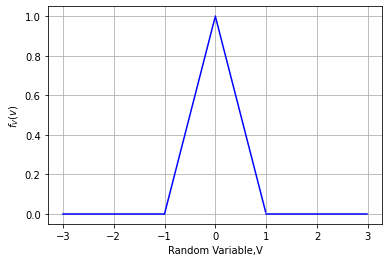
\includegraphics[width=\columnwidth] {solutions/2018/june/50/Assignment_3_Fig_1.png}
    \caption{The PDF of V}
    \label{june2018-50fig:The PDF of V}
\end{figure}

The CDF of V is defined as,
\begin{equation}
    F_V(v) = \Pr\brak{V \le v}
\end{equation}
Now for $ v \le 0 $,
 \begin{align}
    \Pr\brak{V\le v} &=  \int_{-\infty}^{v}f_{V}(v) \,dv  \\
          &=  \int_{-1}^{v} (1+v) \,dv  \\
          &=  \left(\dfrac{v^2}{2}+v \right) \Biggr|_{-1}^{v}  \\
          &=   \left(\left(\dfrac{v^2}{2}+v \right) - \left(\dfrac{1}{2} -1 \right)\right) \\
          &= \dfrac{v^2+2v +1}{2}
\end{align}
Similarly for $v \le 1$,
\begin{align}
    \Pr\brak{V\le v} &=  \int_{-\infty}^{v}f_{V}(v) \,dv  \\
          &=  \dfrac{1}{2} + \int_{0}^{v}(1-v)\,dz  \\
          &=  \dfrac{-v^2+2v+1}{2}
\end{align}

The CDF is as below: 
\begin{align}
\label{june2018-50eq:cdf_v}
F_{V}(v)  = 
\begin{cases}
0 & v < -1
\\
\dfrac{v^2+2v + 1}{2} &  v \le 0
\\
\dfrac{-v^2+2v+1}{2} &  v \le 1
\\
1 & v > 1
\end{cases}
\end{align}

The plot for CDF of $V $ can be observed at figure \ref{june2018-50fig:The CDF of V}\\

\begin{figure}[!ht]
       \centering
    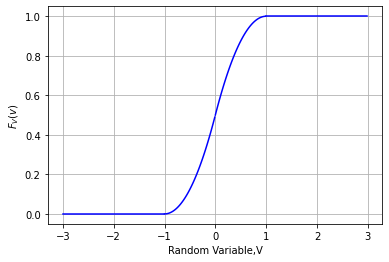
\includegraphics[width=\columnwidth] {solutions/2018/june/50/Assignment_3_Fig_2.png}
    \caption{The CDF of V}
    \label{june2018-50fig:The CDF of V}
\end{figure}

We need  $\pr{Z-W >\frac{1}{2}}$ where $Z = max(X,Y)$ and $W = min(X,Y)$. Now,

\begin{align}
\label{june2018-50eq:pdf_v}
Z-W  = 
\begin{cases}
X-Y & \text{for } X \geq Y
\\
Y-X & \text{for } X < Y
\end{cases}
\end{align}

Therefore,
\begin{align}
    \pr{Z-W >\frac{1}{2}} &= \pr{X-Y>\frac{1}{2},X \geq Y} \nonumber \\
    &+\pr{Y-X > \frac{1}{2}, X < Y}\\
    &= \pr{X-Y>\frac{1}{2}} +\pr{Y-X>\frac{1}{2}}\\
    &= \pr{V > \frac{1}{2}} + \pr{-V > \frac{1}{2}}\\
    &= 1 - \pr{V \leq \frac{1}{2}} + \pr{V < \frac{-1}{2}}\\
    &= 1-F_V(\frac{1}{2}) + F_V(-\frac{1}{2})\\
    &= 1 -\frac{7}{8} + \frac{1}{8}\\
    &= \frac{1}{4}
\end{align}

Hence the correct answer is option (C).

